% Asset ID: FA22FurtherCentreOfMassTikZ-001
% Source: FM2-Chp3-FurtherCentresOfMass-Final.pdf page 14 + teacher transcript
% Related lesson section: #9 Visual Asset Integration; #8.7 Solids of Revolution
% Purpose: Show a solid generated by rotating y=f(x) about the x-axis, with a thin disc at position x.
\documentclass[tikz,border=8pt]{standalone}
\usepackage{amsmath}
\usepackage{xcolor}
\usetikzlibrary{arrows.meta,calc}
\definecolor{canvas}{HTML}{FAF9F6}\definecolor{ivory}{HTML}{FFFFF0}\definecolor{ink}{HTML}{2C2C2E}\definecolor{linegray}{HTML}{E5E5EA}\definecolor{gold}{HTML}{C5A059}\definecolor{softpink}{HTML}{FBEFEF}
\begin{document}
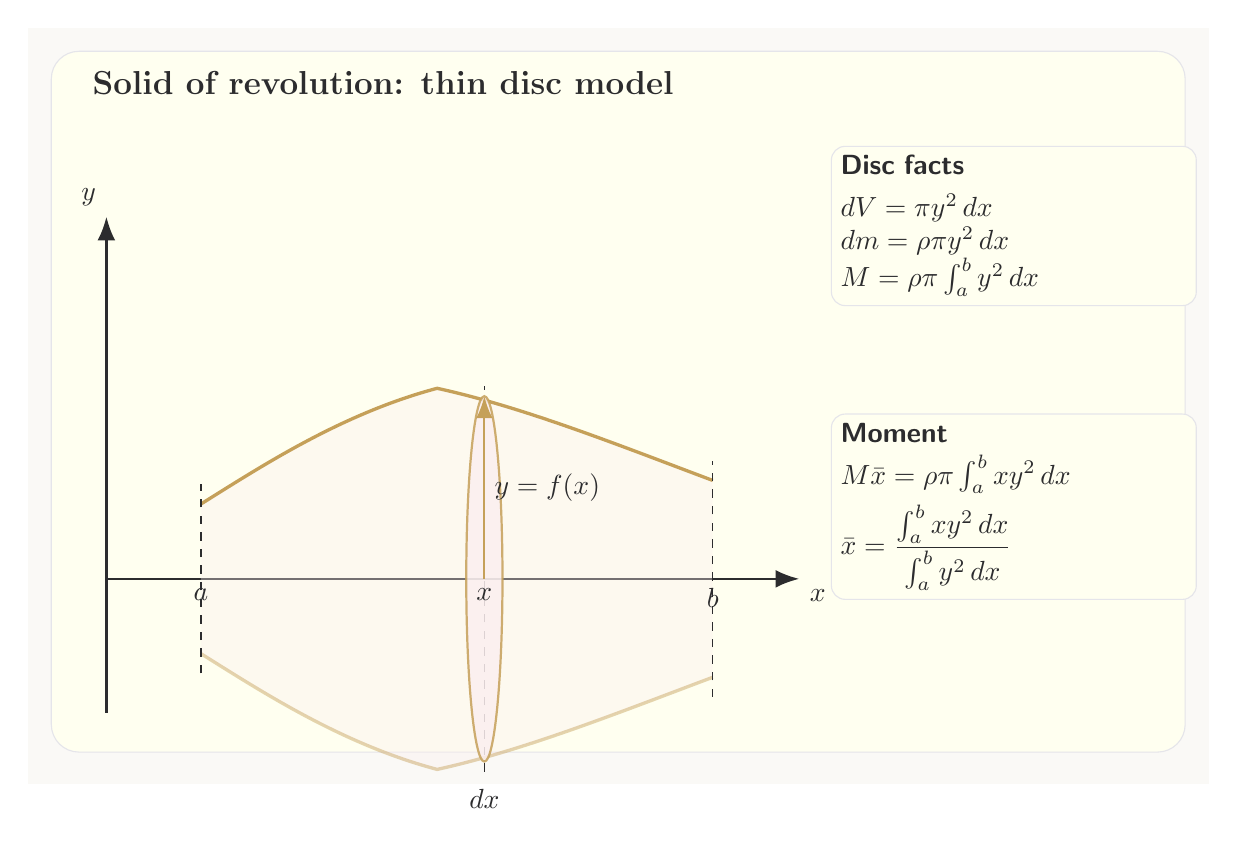
\begin{tikzpicture}[every node/.style={font=\sffamily,text=ink},axis/.style={ink,line width=.9pt,-{Latex[length=3mm]}},main/.style={gold,line width=1.2pt},guide/.style={ink,line width=.45pt,dashed}]
\fill[canvas] (-1,-2.6) rectangle (14,7);
\draw[linegray,fill=ivory,rounded corners=10pt] (-.7,-2.2) rectangle (13.7,6.7);
\node[anchor=west,font=\bfseries\large] at (-.3,6.3){Solid of revolution: thin disc model};
\draw[axis] (0,0)--(8.8,0) node[below right]{$x$};\draw[axis] (0,-1.7)--(0,4.6) node[above left]{$y$};
\path[fill=softpink,opacity=.35] (1.2,.95)..controls (2,1.45) and (3,2.1)..(4.2,2.42)..controls(5.3,2.18) and (6.5,1.7)..(7.7,1.25)--(7.7,-1.25)..controls(6.5,-1.7) and (5.3,-2.18)..(4.2,-2.42)..controls(3,-2.1) and (2,-1.45)..(1.2,-.95)--cycle;
\draw[main] (1.2,.95)..controls (2,1.45) and (3,2.1)..(4.2,2.42)..controls(5.3,2.18) and (6.5,1.7)..(7.7,1.25);
\draw[main,opacity=.45] (1.2,-.95)..controls (2,-1.45) and (3,-2.1)..(4.2,-2.42)..controls(5.3,-2.18) and (6.5,-1.7)..(7.7,-1.25);
\draw[guide] (1.2,-1.2)--(1.2,1.2);\draw[guide] (7.7,-1.5)--(7.7,1.5);\node[below] at (1.2,0){$a$};\node[below] at (7.7,0){$b$};
\draw[guide] (4.8,-2.45)--(4.8,2.45);\draw[fill=softpink,draw=gold,line width=.8pt,opacity=.85] (4.8,0) ellipse (.23 and 2.32);\draw[gold,-{Latex[length=2.8mm]},line width=.8pt] (4.8,0)--(4.8,2.32) node[midway,right]{$y=f(x)$};\node[below] at (4.8,0){$x$};\node[below] at (4.8,-2.55){$dx$};
\node[draw=linegray,fill=ivory,rounded corners=5pt,text width=4.4cm,anchor=north west] at (9.2,5.5){\textbf{Disc facts}\\[3pt]$dV=\pi y^2\,dx$\\$dm=\rho\pi y^2\,dx$\\$M=\rho\pi\int_a^b y^2\,dx$};
\node[draw=linegray,fill=ivory,rounded corners=5pt,text width=4.4cm,anchor=north west] at (9.2,2.1){\textbf{Moment}\\[3pt]$M\bar{x}=\rho\pi\int_a^bxy^2\,dx$\\[3pt]$\displaystyle\bar{x}=\frac{\int_a^bxy^2\,dx}{\int_a^by^2\,dx}$};
\end{tikzpicture}
\end{document}
